\section*{Задание 1}
Запустить среду Visual Prolog5.2. Настроить утилиту TestGoal. Запустить тестовую программу, проанализировать реакцию системы и множество ответов. Разработать свою программу - «Телефонный справочник». Протестировать работу программы.

\subsection*{Решение}
\begin{lstinputlisting}[label=third,caption=Решение задания №1, language=lisp, firstline=12, lastline=23]{../lab_11.pro}
\end{lstinputlisting}

\section*{Задание 2}
Составить программу – базу знаний, с помощью которой можно определить, например, множество студентов, обучающихся в одном ВУЗе и их телефоны. Студент может одновременно обучаться в нескольких ВУЗах. Привести примеры возможных вариантов вопросов и варианты ответов (не менее 3-х). Описать порядок формирования вариантов ответа.

Исходную базу знаний сформировать с помощью только фактов.

*Исходную базу знаний сформировать, используя правила.

**Разработать свою базу знаний (содержание произвольно).

\subsection*{Решение}

\begin{lstinputlisting}[label=third,caption=Решение задания №1, language=lisp, firstline=12, lastline=38]{../lab_11_2.pro}
\end{lstinputlisting}

\section*{Задание 3}
Составить программу, т.е. модель предметной области – базу знаний, объединив в ней
информацию – знания:

\begin{itemize}
	\item «Телефонный справочник»: Фамилия, №тел, Адрес – структура (Город,
	Улица, №дома, №кв),
	\item «Автомобили»: Фамилия\_владельца, Марка, Цвет, Стоимость, и др.,
	\item «Вкладчики банков»: Фамилия, Банк, счет, сумма, др.
\end{itemize}
Владелец может иметь несколько телефонов, автомобилей, вкладов (Факты).
Используя правила, обеспечить возможность поиска:
\begin{enumerate}
	\item По № телефона найти: Фамилию, Марку автомобиля, Стоимость автомобиля
	(может быть несколько),Используя сформированное в пункте а) правило, по № телефона найти:
	только Марку автомобиля (автомобилей может быть несколько)
	\item Используя простой, не составной вопрос: по Фамилии (уникальна в городе, но в
	разных городах есть однофамильцы) и Городу проживания найти:
	Улицу
	проживания, Банки, в которых есть вклады и №телефона
\end{enumerate}

\subsection*{Решение}

\begin{lstinputlisting}[label=third,caption=Решение задания №3, language=lisp, firstline=0, lastline=41]{../lab_12_1.pro}
\end{lstinputlisting}

\newpage
\begin{figure}[H]
	\caption{Таблица к заданию 1а.}
	\begin{center}
		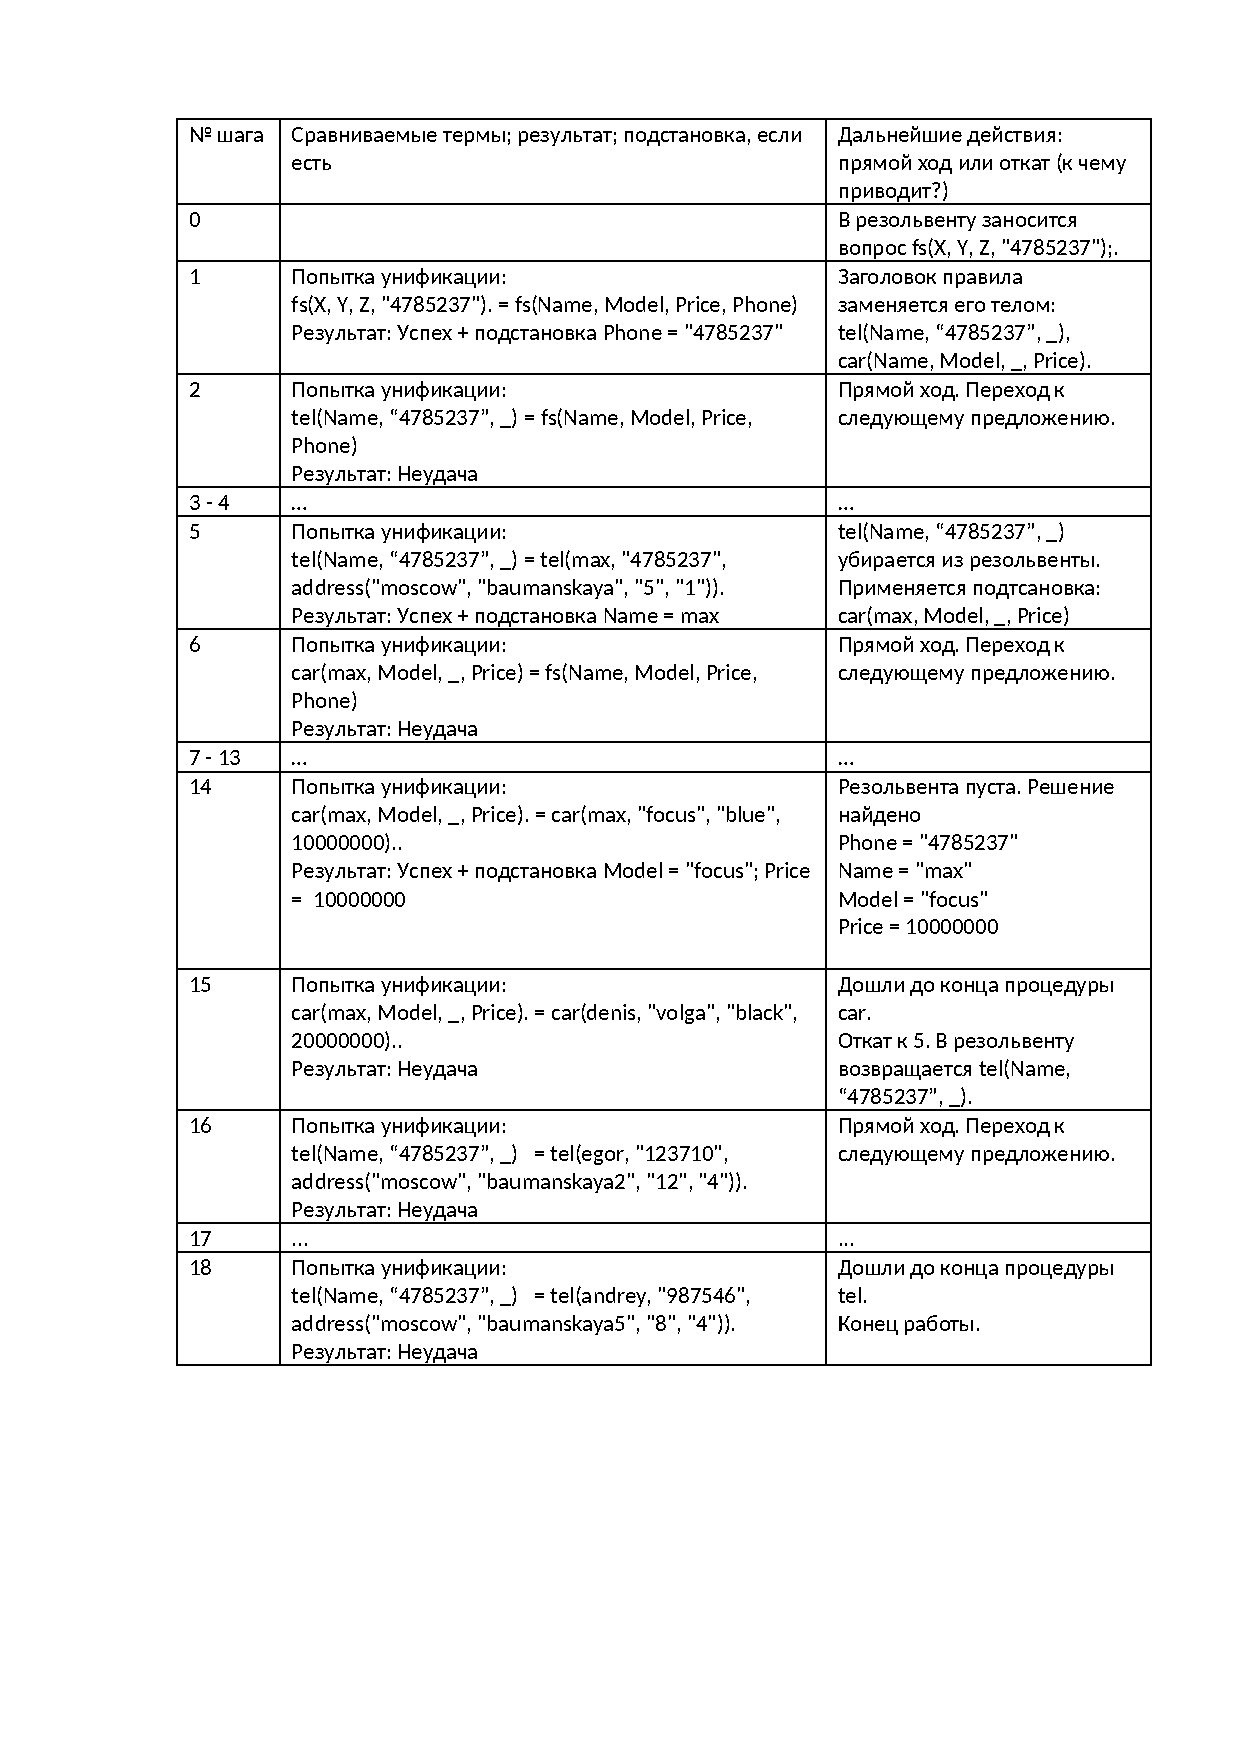
\includegraphics[scale=0.85]{img/12.1a.pdf}
	\end{center}

\end{figure}

\newpage
\begin{figure}[H]
	\caption{Таблица к заданию 1b.}
	\begin{center}
		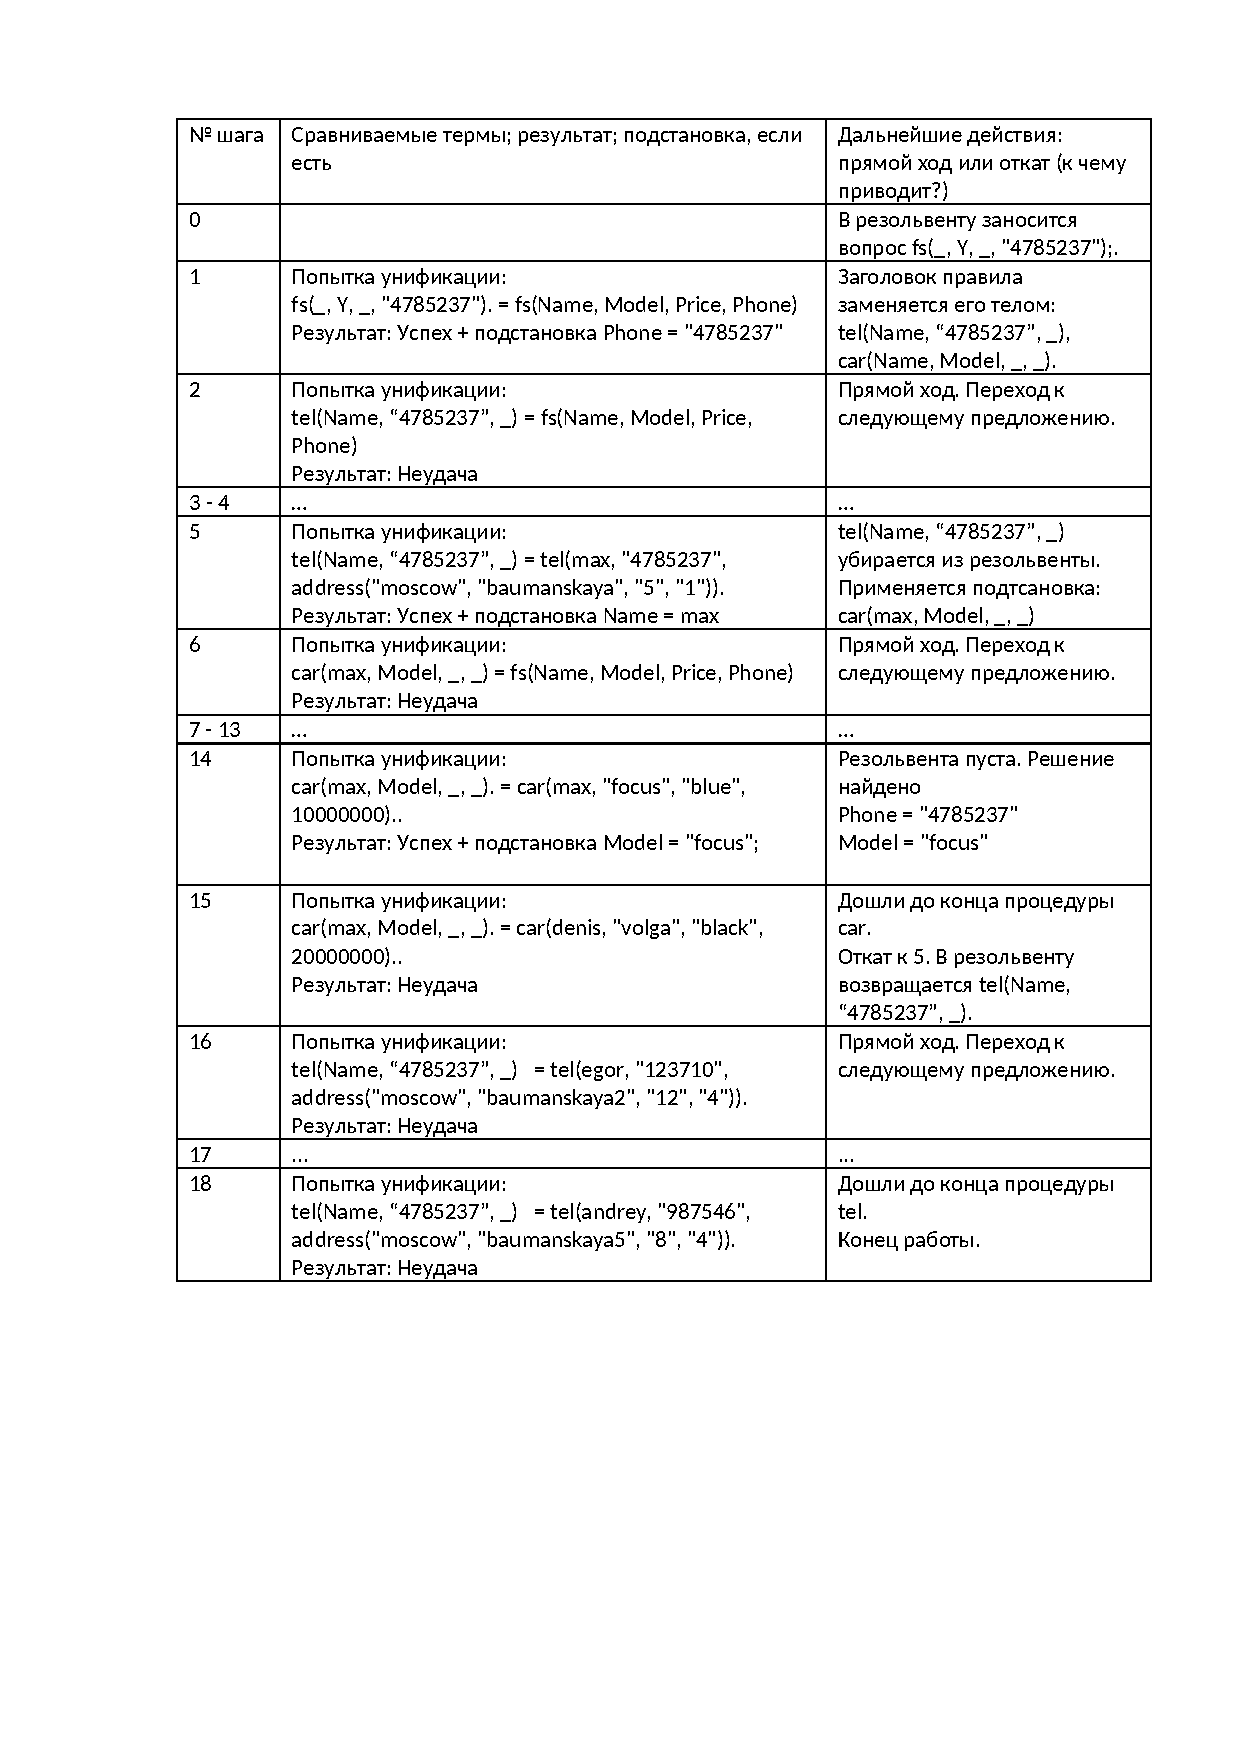
\includegraphics[scale=0.85]{img/12.1b.pdf}
	\end{center}
\end{figure}

\section*{Задание 4}
Используя конъюнктивное правило и простой вопрос, обеспечить возможность поиска: По Марке и Цвету
автомобиля найти Фамилию, Город, Телефон и Банки, в которых владелец автомобиля имеет вклады.

\begin{lstinputlisting}[label=third,caption=Решение задания №4, language=lisp, firstline=0, lastline=41]{../lab_12_2.pro}
\end{lstinputlisting}

\textbf{Ответ 1}

No solution

\textbf{Ответ 2}

Name=denis, City=moscow, Phone=167765, Bank=raif

1 Solution

\textbf{Ответ 3}

Name=max, City=moscow, Phone=4785237, Bank=tinkoff

Name=max, City=moscow, Phone=4785237, Bank=sber

Name=egor, City=moscow, Phone=123710, Bank=sber

3 Solutions

\newpage
\begin{figure}[H]
	\caption{Таблица к заданию.}
	\begin{center}
		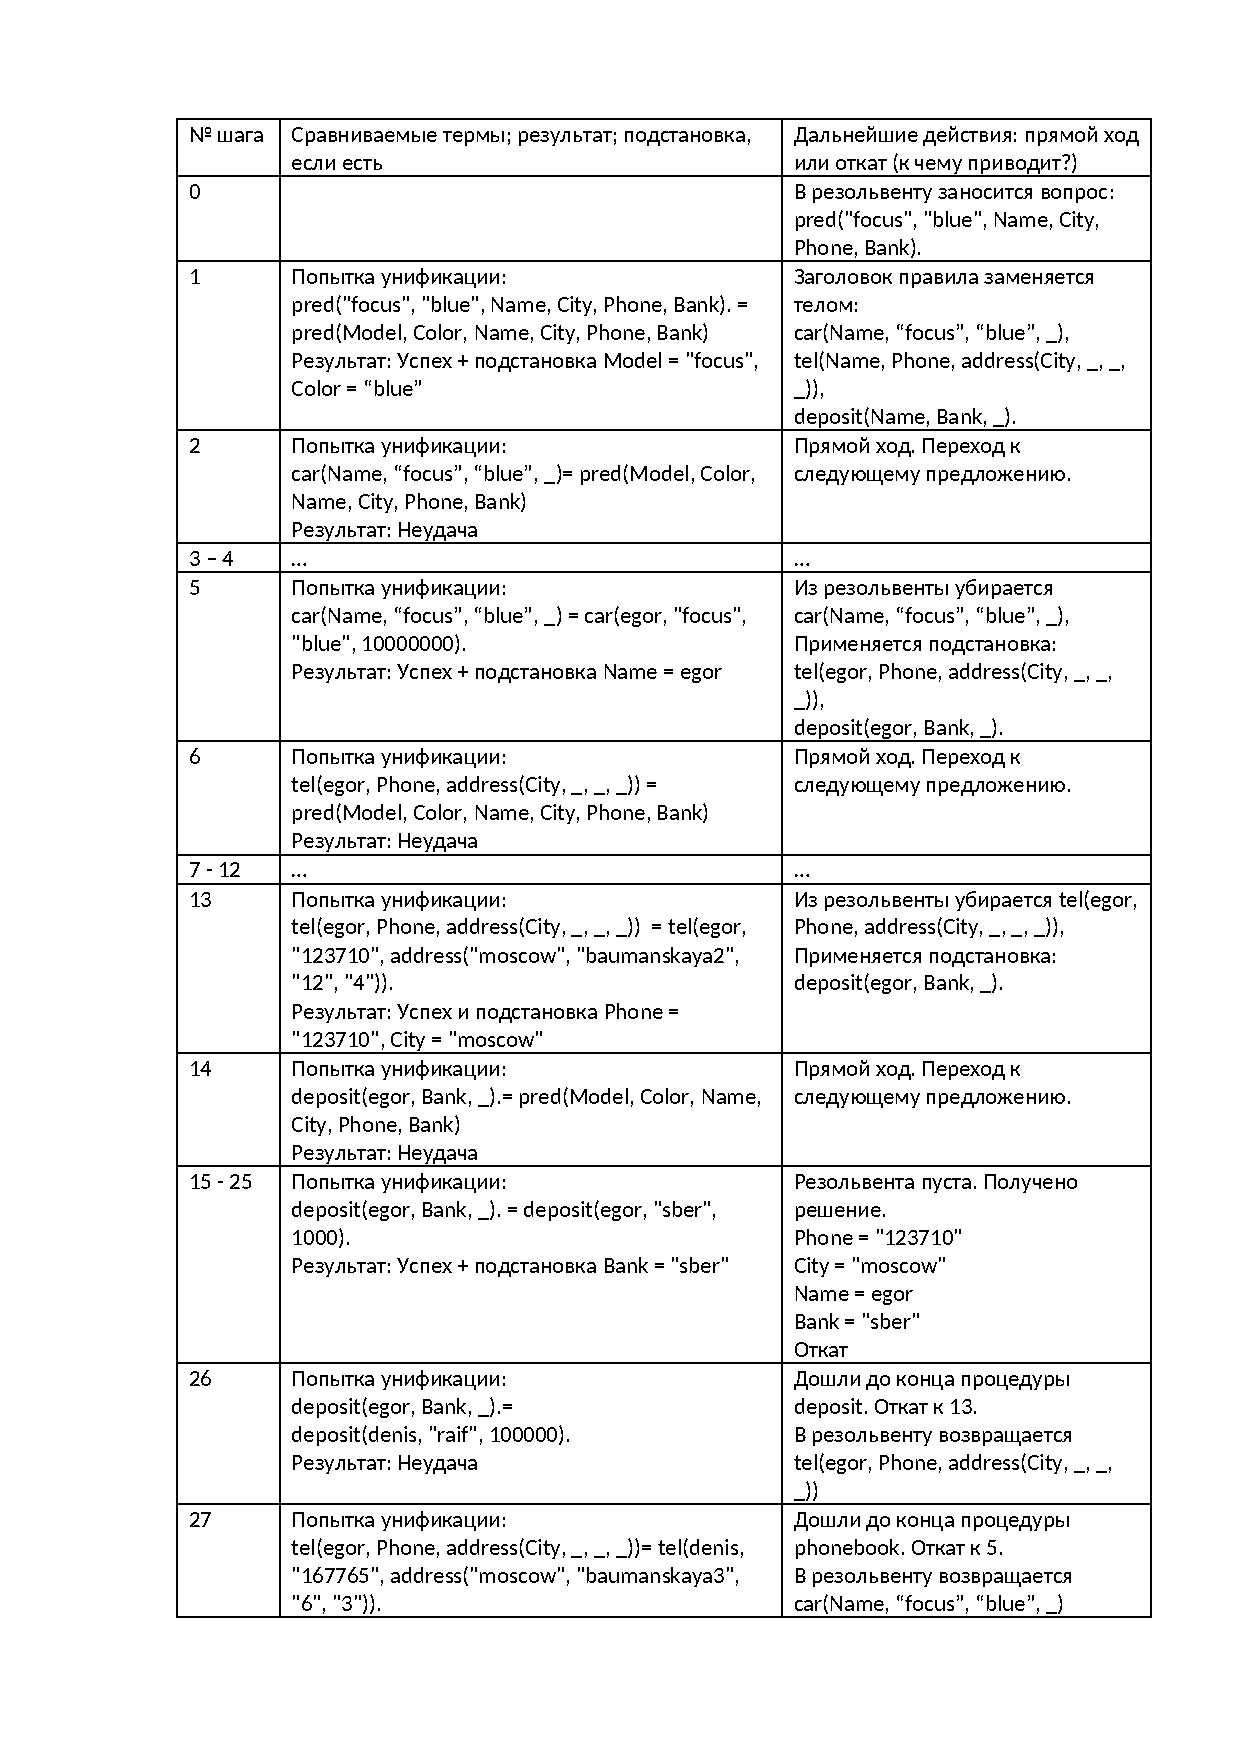
\includegraphics[scale=0.85]{img/13.1.pdf}
	\end{center}
	
\end{figure}

\newpage
\begin{figure}[H]
	\begin{center}
		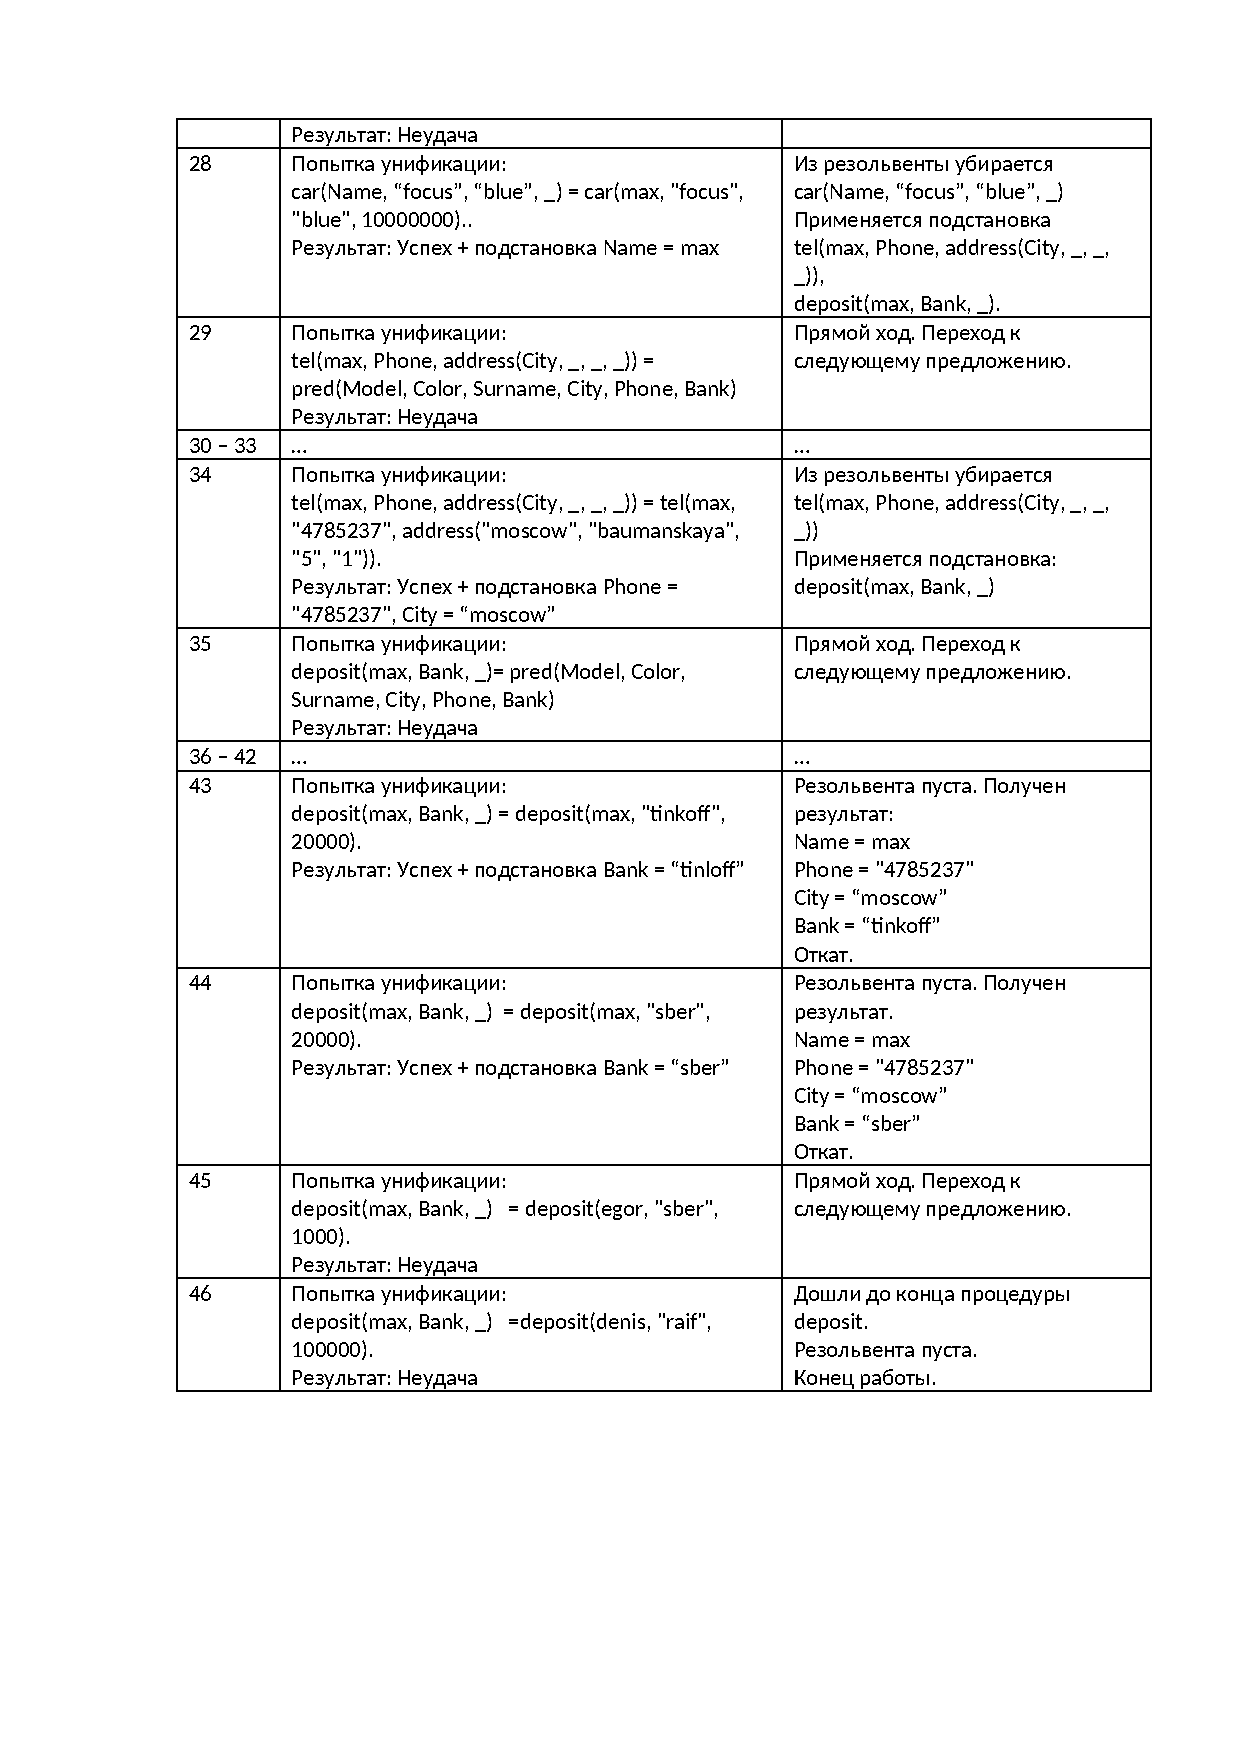
\includegraphics[scale=0.85]{img/13.2.pdf}
	\end{center}
\end{figure}


\section*{Теоретическая часть}

\subsection*{Как представляется программа на языке Prolog?}

Программа на языке Prolog состоит из базы знаний --- фактов и правил. Цель системы --- дать ответ "да"{} на поставленный в разделе goal вопрос, используя знания. Или "нет"{}, если невозможно дать ответ "да"{}.

\subsection*{Структура программы}

Программа на Prolog состоит из разделов. Каждый раздел начинается со своего 
заголовка. Структура программы:

\begin{itemize}
	\item директивы компилятора — зарезервированные символьные константы
	\item CONSTANTS — раздел описания констант
	\item DOMAINS — раздел описания доменов
	\item DATABASE — раздел описания предикатов внутренней базы данных
	\item PREDICATES — раздел описания предикатов
	\item CLAUSES — раздел описания предложений базы знаний
	\item GOAL — раздел описания внутренней цели (вопроса)
\end{itemize}

В программе не обязательно должны быть все разделы.

\subsection*{Работа программы}

Ответ на поставленный вопрос система дает в логической форме -- «Да» или «Нет». Цель системы состоит в том, чтобы на поставленный вопрос найти возможность, исходя из базы знаний, ответить «Да». Вариантов ответить «Да» на поставленный вопрос может быть несколько. В нашем случае система настроена в режим получения всех возможных вариантов ответа. При поиске ответов на вопрос рассматриваются альтернативные варианты и находятся все возможные решения (методом проб и ошибок) -- множества значений переменных, при которых на поставленный вопрос можно ответить -- «Да».

Для выполнения логического вывода используется механизм унификации, встроенный в систему.
Унификация -- операция, которая позволяет формализовать процесс логического вывода. С практической точки зрения -- это основной вычислительный шаг, с помощью которого происходит:
\begin{itemize}
	\item Двунаправленная передача параметров процедурам,
	\item Неразрушающее присваивание,
	\item Проверка условий (доказательство).
\end{itemize}

\subsection*{4. Что такое терм?}

Терм - основной элемент языка Prolog. Терм – это:

\begin{enumerate}
	\item Константа: 
	\begin{itemize}
		\item Число (целое, вещественное),
		\item Символьный атом (комбинация символов латинского алфавита, цифр и символа подчеркивания, начинающаяся со строчной буквы),
		\item Строка: последовательность символов, заключенных в кавычки.
	\end{itemize}
	\item Переменная:
	\begin{itemize}
		\item Именованная – обозначается комбинацией символов латинского алфавита, цифр и символа подчеркивания, начинающейся с прописной буквы или символа подчеркивания,
		\item Анонимная  - обозначается символом подчеркивания
	\end{itemize}
	\item Составной терм:
	Это средство организации группы отдельных элементов знаний в единый  объект,  синтаксически представляется: f(t1, t2, …,tm), где f -  функтор (отношение между объектами), t1, t2, …,tm – термы, в том  числе  и составные.
\end{enumerate}

\subsection*{5. Что такое предикат в матлогике (математике)?}

Предикат в математической логике - это утверждение, высказанное о субъекте. Предикат является функцией со значениями {0, 1} (истина/ложь), определенной на некотором множестве параметров. Предикат называют n-арным, если он определен на n-ой декартовой степени множества М.

\subsection*{6. Что описывает предикат в Prolog?}

Предикат в Prolog описывает отношение между аргументами процедуры. Процедурой в Prolog является совокупность всех правил, описывающих определенное отношение.

\subsection*{7. Назовите виды предложений в программе и приведите примеры таких предложений из вашей программы. Какие предложения являются основными, а какие - не основными? Каковы: синтаксис и семантика (формальных смысл) этих предложений (основных и неосновных)?}

В Prolog есть два типа предложений: правила и факты. Правило имеет вид: $A$ :- $B_{1}$,... ,$B_{n}$. 
A называется заголовком правила, а $B_{1}$,...,$B_{n}$ – телом правила. Заголовок содержит некоторое знание, а тело - условие истинности этого знания. Факт является частным случаем правила - в нем отсутствует тело. 

\begin{itemize}
	\item Пример факта из программы: \emph{car(anton, "x6", "red", 10000000). }
	\item Пример правила из программы: \emph{fs(Name, Model, Price, Phone):- tel(Name, Phone, \_),  car(Name, Model,  \_, Price). }
\end{itemize}


Основными называются предложения, не содержащие переменных. Предложения, содержащие переменные называются неосновными.\\

Синтаксис предложения: заголовок(составной терм) :- тело(один или последовательность термов). Предложения используются для формирования базы знаний о некоторой предметной области.

\subsection*{8. Каковы назначение, виды и особенности использования переменных в программе на Prolog? Какое предложение БЗ сформулировано в более общей - абстрактной форме: содержащее или не содержащее переменных?}

Переменные предназначены для обозначения некоторого неизвестного объекта предметной области. Переменные бывают именованными и анонимными. Именованные переменные уникальны в рамках предложения, а анонимная переменная – любая уникальна. В разных предложениях может использоваться одно имя переменной для обозначения разных объектов.

В ходе выполнения программы выполняется связывание переменных с различными объектами, этот процесс называется конкретизацией. Это относится только к именованным переменным. Анонимные переменные не могут быть связаны со значением.

В более общей форме сформулировано предложение, содержащее переменные, так как заранее неизвестно, каким объектом будет конкретизирована переменная.

\subsection*{9. Что такое подстановка?}

Пусть дан терм: $А(X_1, X_2,  \dots ,X_n)$.
Подстановка - множество пар, вида: $\{X _ i = t _ i\}$, где $X_i$ –   переменная, а $t_i$ –  терм.	